\documentclass[tikz,border=3pt]{standalone}
\usepackage[utf8]{inputenc}
\usepackage[T1]{fontenc}
\usepackage{lmodern}
\renewcommand{\familydefault}{\sfdefault}
\usepackage{sansmath}\sansmath
\usepackage{chemfig}
\usepackage{pgfplots}\pgfplotsset{compat=1.18,/pgf/number format/use comma,/pgf/number format/1000 sep={.}}
\usetikzlibrary{arrows.meta,calc,positioning,decorations.pathmorphing,patterns}
% paleta del sitio
\definecolor{nar}{HTML}{E8680C}\definecolor{narc}{HTML}{FFB35C}\definecolor{hielo}{HTML}{FFF3E8}
\definecolor{tinta}{HTML}{1D1D1F}\definecolor{gris}{HTML}{6E6E73}\definecolor{lila}{HTML}{7C5CF0}
\definecolor{azul}{HTML}{2F6FD6}\definecolor{menta}{HTML}{17A673}\definecolor{coral}{HTML}{E8342A}
\begin{document}
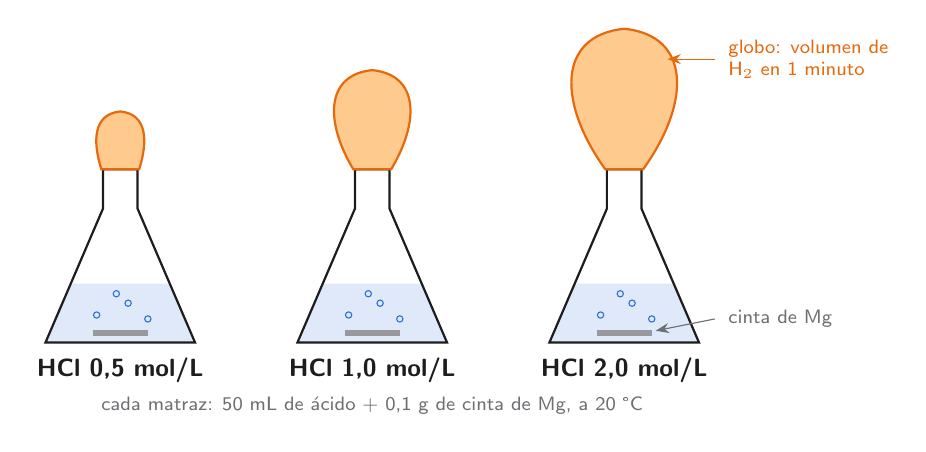
\begin{tikzpicture}[font=\small]
% matraz: base ancha, cuello angosto; #1 = x, #2 = radio del globo, #3 = rotulo
\newcommand{\matraz}[3]{%
  \begin{scope}[shift={(#1,0)}]
    \fill[azul!15] (-0.95,0) -- (0.95,0) -- (0.62,0.75) -- (-0.62,0.75) -- cycle;
    \draw[tinta,thick] (-0.95,0) -- (0.95,0) -- (0.22,1.7) -- (0.22,2.2) -- (-0.22,2.2) -- (-0.22,1.7) -- cycle;
    \fill[gris!70] (-0.35,0.08) rectangle (0.35,0.16);
    \foreach \b in {(-0.3,0.35),(0.1,0.5),(0.35,0.3),(-0.05,0.62)} \draw[azul,thin] \b circle (0.04);
    \fill[narc!70,draw=nar,thick] (-0.24,2.2) .. controls (-#2,2.2+#2) and (-#2,2.2+2*#2) .. (0,2.2+2.1*#2)
       .. controls (#2,2.2+2*#2) and (#2,2.2+#2) .. (0.24,2.2) -- cycle;
    \node[font=\small\bfseries,text=tinta] at (0,-0.35) {#3};
  \end{scope}}
\matraz{0}{0.35}{HCl 0,5 mol/L}
\matraz{3.2}{0.6}{HCl 1,0 mol/L}
\matraz{6.4}{0.85}{HCl 2,0 mol/L}
\node[font=\scriptsize,text=gris] at (3.2,-0.8) {cada matraz: 50 mL de ácido + 0,1 g de cinta de Mg, a 20 °C};
% leyendas
\node[anchor=west,font=\scriptsize,text=nar,align=left] at (7.6,3.6) {globo: volumen de\\H$_2$ en 1 minuto};
\draw[-{Stealth},nar] (7.55,3.6) -- (6.95,3.6);
\node[anchor=west,font=\scriptsize,text=gris,align=left] at (7.6,0.3) {cinta de Mg};
\draw[-{Stealth},gris] (7.55,0.3) -- (6.8,0.15);
\end{tikzpicture}
\end{document}
